\documentclass[10pt]{article}
\usepackage[a4paper,margin=2.2cm]{geometry}
\usepackage[T1]{fontenc}
\usepackage[utf8]{inputenc}
\usepackage{lmodern}
\usepackage{amsmath,amssymb}
\usepackage{booktabs}
\usepackage{graphicx}
\usepackage{pgfplots}
\pgfplotsset{compat=1.16}
\usepackage{xcolor}
\usepackage[hidelinks]{hyperref}
\usepackage{caption}
\captionsetup{font=small,labelfont=bf}
\newcommand{\tps}{tok/s}

\title{\textbf{SR-HPM: Speculative Verification on the CPU}\\[2pt]
\large Fast decoding of dense LLMs larger than GPU memory on consumer hardware}
\author{Javitax47\thanks{Code, data and lab notes: \url{https://github.com/Javitax47/sr-hpm}.
The experiments, code and text were produced with the assistance of an AI coding agent (Claude, Anthropic)
under the author's direction.}}
\date{October 2026}

\begin{document}
\maketitle

\begin{abstract}
A dense 27B-parameter model quantized to ${\sim}3.5$ bits does not fit in the 6\,GB of a laptop GPU. Partial offload
leaves most weights in system RAM, and decoding becomes bound by reading them once per generated token. Speculative
decoding should amortize that read over several tokens, but on the CPU path of llama.cpp verifying $M$ drafted tokens
costs 2--4$\times$ a single token, so drafters barely help. We present SR-HPM, a patch to llama.cpp and a launcher
that make verification on the CPU nearly memory-flat (4 tokens for $1.1$--$1.2\times$ the cost of one) and then remove
the remaining costs of the pipeline one measurement at a time: cost-aware layer placement, a lossless 4-bit
re-encoding of grid-quantized weights, lazy rollback snapshots for hybrid recurrent models, a split prompt-processing
path, co-verification by the otherwise idle GPU reading weights from RAM over PCIe, large pages, and kernel-aware
re-quantization. On Qwen3.8-27B with an RTX 3060 Laptop and a Ryzen 7 5800H, greedy decoding goes from
2.7\,\tps{} (stock llama.cpp with the same drafter) to 9.6--10.2\,\tps{} with identical output, and
${\sim}10.4$\,\tps{} with an opt-in relaxed acceptance that costs 0.018\,nats per token. We also report about twenty
ideas that did \emph{not} work---draft trees, rerankers, activation sparsity, layer dropping, 2-bit layers with
low-rank correction among them---each with the cheap experiment that refuted it, and identify the two walls that remain:
RAM bandwidth in the typical 4-token pass, and the drafter's acceptance rate.
\end{abstract}

\section{Introduction}

Running a model whose weights exceed GPU memory is the common case on consumer machines. llama.cpp~\cite{llamacpp}
splits such a
model by layers between GPU and CPU; for dense models the CPU part dominates, and one decoding step reads every
CPU-resident weight from DRAM. On our reference laptop (dual-channel DDR4-3200, ${\sim}38$\,GB/s measured) the
${\sim}9$\,GB that do not fit in VRAM bound decoding to a few tokens per second.

Speculative decoding~\cite{leviathan,chen,eagle} turns this around in principle: a cheap drafter proposes several tokens
and the target model verifies them in one pass, so one read of the weights yields several tokens. The premise is that
verifying $M$ tokens costs about as much as one, which holds on GPUs. It does not hold on the CPU path of
llama.cpp: its quantized matrix kernels re-decode each weight block for every token, so a 4-token pass costs
2.1--2.7$\times$ a 1-token pass (Table~\ref{tab:kernel}). With a strong drafter (DFlash2) stock llama.cpp reaches
2.7\,\tps{} on Qwen3.8-27B.

SR-HPM---\emph{Speculative verification on RAM-resident weights for Heterogeneous PC Memory}---starts from a
verification kernel that decodes each block once for all tokens, and then follows the cost of a decoding step wherever
it goes.\footnote{The acronym comes from the project's original proposal, \emph{Speculative Residual $\cdot$
Hierarchical Precision Memory}; its audit refuted several components, and the name was kept and re-read to describe
what survived.} Our contributions are:
\begin{itemize}
\item small-batch CPU kernels for the quantization formats of modern dynamic quants, including a lossless 4-bit
re-encoding (C4) that replaces grid lookups by a single shuffle, sign-free paths for offset-coded types, and a
paired layout for IQ4\_XS (\S\ref{sec:kernels});
\item rollback machinery for hybrid recurrent models (gated delta networks) that keeps two full states per pass and
replays the rest exactly from rank-1 records, and a split prompt-processing path that keeps those snapshots exact at
GPU speed (\S\ref{sec:recurrent});
\item co-verification by the discrete GPU, which reads a share of the CPU layers' weights directly from pinned RAM
over PCIe while the CPU computes the rest (\S\ref{sec:dgpu});
\item placement, drafting, quantization and system choices, each justified by an A/B measurement, and a launcher
that applies them to any dense GGUF model (\S\ref{sec:system});
\item a catalogue of refuted ideas with the experiments that refuted them (\S\ref{sec:negative}), and an analysis of
where the remaining time goes.
\end{itemize}

\section{Setting and methodology}

\paragraph{Hardware and model.} Laptop with an RTX 3060 Laptop GPU (6\,GB, PCIe~3.0~x8), Ryzen~7~5800H (8 Zen~3 cores,
AVX2, no VNNI), 32\,GB DDR4-3200, Windows~11. Target: Qwen3.8-27B, a hybrid model with 64 layers (48 gated-delta-net
recurrent layers, 16 full-attention layers), quantized from Unsloth's UD-Q3\_K\_XL dynamic recipe (12.2\,GB) and later
from our own kernel-aware mix (12.4\,GB). Drafter: DFlash2 (block 8, a 16-candidate selector lattice), Q4\_K\_M, on
the GPU.

\paragraph{Metrics.} Decode speed is the mean over 10 fixed prompts (code, math, prose, translation; Spanish and
English), 200 greedy tokens each, with thinking disabled. A hash of the outputs certifies exactness: changes that
must not alter the output are rejected if the hash changes. Quality is the KL divergence to the Q8\_0 model on
$16\times512$ tokens of a held-out corpus (\texttt{llama-perplexity --kl-divergence}), with the fraction of positions
where the top token agrees. $\tau$ is the number of tokens produced per verification pass.

\paragraph{Noise.} The laptop drifts by $\pm10\%$ with temperature and background load. Every comparison is made in
pairs within one session (A~B~A~B); we report both runs. Differences inside the pair spread are reported as ties.

\section{Small-batch verification kernels}\label{sec:kernels}

\begin{table}[t]
\centering\small
\begin{tabular}{rcccc}
\toprule
$M$ (tokens) & our kernel (ms) & cost vs $M{=}1$ & llama.cpp Q3\_K & llama.cpp Q4\_0 \\
\midrule
1 & 1.62 & 1.00 & 1.00 & 1.00 \\
2 & 1.75 & 1.08 & 1.53 & 1.28 \\
4 & 1.92 & 1.18 & 2.73 & 2.05 \\
8 & 2.87 & 1.77 & 3.89 & 3.30 \\
\bottomrule
\end{tabular}
\caption{Cost of one $17408\times5120$ 4-bit matrix product (does not fit in L3) for $M$ tokens, 8 threads. The
first kernel prototype already makes 4 tokens cost 1.18$\times$ one; llama.cpp's CPU path costs 2--2.7$\times$.}
\label{tab:kernel}
\end{table}

The kernel family \texttt{GGML\_SRV} decodes each 256-weight super-block once into signed 8-bit values and applies it to
the $M\le8$ activation rows held in registers or L1 (\texttt{vpmaddubsw} on $|w|$ and sign-adjusted activations,
then \texttt{vpmaddwd} and 32-bit accumulation). Activations are quantized per row to 8 bits with per-block scales,
bit-identically to ggml's Q8\_K, so the result equals stock llama.cpp.

\paragraph{C4: lossless 4-bit re-encoding of grid quants.} IQ3\_S and IQ3\_XXS store indices into a 512- or
256-entry grid of 4 values each; decoding needs one gather per 4 weights, which dominates once the data is in cache.
Within a 32-weight sub-block those grids use at most 16 distinct magnitudes, so we re-encode the weights losslessly as
4-bit codes plus a 16-entry table and decode with one \texttt{pshufb}: 1.5--1.8$\times$ faster, 4.375 bits per weight.

\paragraph{Sign-free paths.} Q3\_K, C4 and Q6\_K store $w+o$ with a constant offset. Multiplying the unsigned code
directly and subtracting $o\cdot\sum x$ per group removes the per-token sign step (one instruction of five);
the group sums come from one vector per super-block.

\paragraph{Paired IQ4\_XS.} Loading two 32-weight sub-blocks per 32-byte load and permuting the activations once per
pass instead of shuffling weights per block cuts IQ4\_XS (53\% of the CPU bytes) by 5--7\%.

\paragraph{The wall.} With these kernels the CPU reads IQ4\_XS at 35\,GB/s for 4 tokens, against a measured RAM
ceiling of 38--41\,GB/s; with 8 tokens it is compute-bound at ${\sim}20$\,GB/s. A synthetic peak benchmark puts the
Zen~3 compute ceiling at 1.48 cycles per 32 weights and token with the sign step and 1.10 without, against 2.0--2.3
in the real kernel.

\section{Rollback for hybrid recurrent models}\label{sec:recurrent}

Speculative decoding must undo rejected tokens. For attention layers this means truncating the KV cache; for
recurrent layers llama.cpp keeps $K=n_\text{draft}+1$ snapshots of the state per layer (a $128\times128$ matrix per
head, 3\,MB per layer) and writes all of them every pass---400--800\,MB of writes per pass on Qwen3.8-27B.

\paragraph{Direct and lazy snapshots.} We first write the snapshots straight into the cache from the CPU kernel instead
of through the op output and a copy ($+6\%$). Then we observe that the gated delta rule
$S_t = g_t S_{t-1} + k_t \delta_t^\top$ is a rank-1 update: keeping two full states (the newest and the oldest slot) and
the vectors $(k_t,\delta_t,g_t)$ of the tokens in between (${\sim}1$\,KB per head) allows an exact replay of any
intermediate state when a rollback actually happens. The output hash is unchanged and decoding is 4\% faster.

\paragraph{Split prompt processing.} With rollback enabled, prompt processing was 35\% slower than without a drafter.
Removing the drafter's injection or feature extraction changed nothing; forcing rollback snapshots without a drafter
reproduced the loss exactly. Two independent costs: (i) 8 strided copies per layer of the convolution state out of the
whole ubatch (${\sim}5$\,s per 3.6k-token prompt), replaced by one gather of the last $K+2$ columns; (ii) the lazy
recurrent op exists only on the CPU, where it runs token by token, while the regular op is offloaded to the GPU for
large batches and runs in chunks. For prompt ubatches the lazy op now processes only the first token (rebuilding the
state of a pending rollback) and the regular op the rest, writing full snapshots. Prompt processing goes from 98 to
132\,\tps{} (145 without a drafter), with identical output.

\section{dGPU co-verification over PCIe}\label{sec:dgpu}

During the CPU part of a pass---most of it---the GPU is idle. We let it compute the first rows of every IQ4\_XS and
Q3\_K product of the CPU layers, reading a pinned copy of those rows from RAM over PCIe with zero-copy loads (one
warp per row streams the row through shared memory with consecutive 4-byte loads), while the CPU threads compute the
remaining rows. Measured alone, PCIe~3.0~x8 delivers 6.7\,GB/s, and with the CPU kernel running concurrently the two
add up to 29.3\,GB/s without slowing the CPU. In the model the gain depends on $M$: with 4 tokens the CPU already reads
35\,GB/s, and PCIe reads only compete for the same DRAM (890$\to$1120\,$\mu$s per product); from 6 tokens the CPU is
compute-bound and the GPU's rows are a net gain ($-15\%$ per product at $M=8$). With a per-$M$ share table
($0$ up to 5 tokens, then 12\%, 16\%, 20\%) the pass is 2--4\% shorter. The GPU rows use float activations and are
slightly more precise than the CPU's 8-bit path.

\section{System-level choices}\label{sec:system}

\paragraph{Placement.} VRAM buys CPU time, not bytes: we rank layers by measured CPU seconds per byte of their tensor
types and put the best contiguous range on the GPU (every CPU$\leftrightarrow$GPU boundary costs a synchronization),
plus the output head when the drafter shares it. llama.cpp's op offload sent every CPU layer's normalization to the GPU
(64 boundaries per token); offloading only large-batch products restores 4 boundaries.

\paragraph{Adaptive drafting.} Because 4-token verification is nearly free and 8-token verification is not, we always
keep 3 drafted tokens and extend up to 7 only while the drafter's selector probability stays $\ge0.9$
($\tau$ 3.25$\to$4.2, $+7$--$10\%$). Choosing the length by expected value from the measured cost curve ties.

\paragraph{GPU keep-alive and large pages.} Between bursts the driver drops the GPU to a low clock state; a 1-warp spin
kernel on a separate stream keeps it up ($+0$--$5\%$, drafter 19$\to$11\,ms). With the ``Lock pages in memory'' right,
8\,GB of CPU weights live on 2\,MB pages, which removes most TLB walks of the 8.8\,GB read per pass. Measured in two
pairs: $+10\%$ (9.24 vs 8.40\,\tps) and a tie (8.37 vs 8.47), with identical output---a gain of 0--10\% that the
noise of this session could not pin down.

\paragraph{Kernel-aware quantization.} The CPU path reads IQ3 through C4 at 4.375\,bpw---more bytes than IQ4\_XS
(4.25) for less quality---while Q3\_K is read natively at 3.44\,bpw. Starting from the dynamic recipe, rewriting
only the CPU layers' IQ3 tensors gives two operating points: \emph{quality} (IQ3$\to$IQ4\_XS: KLD 0.0427$\to$0.0345 at
the same speed) and \emph{speed} (FFN IQ3$\to$Q3\_K, attention IQ3$\to$IQ4\_XS: same KLD, $-6.6\%$ CPU bytes,
$+5.7\%$).

\paragraph{Relaxed acceptance (opt-in).} At the position where a draft breaks, the drafted token is often the target's
second choice with a similar probability. Accepting a drafted token whose target logit is within $\delta$ nats of the
best one yields $+6\%$ at $\delta=1$ for 0.018\,nats per token given up---less than half of what the quantization
already costs (Table~\ref{tab:relax}).

\begin{table}[t]
\centering\small
\begin{tabular}{rcccc}
\toprule
$\delta$ & \tps & $\tau$ & acceptance & cost (nats/token) \\
\midrule
0 (exact) & 9.80 & 4.08 & 0.728 & 0 \\
0.5 & 9.85 & 4.13 & 0.756 & 0.004 \\
1 & 10.40 & 4.45 & 0.807 & 0.018 \\
2 & 10.70 & 4.67 & 0.841 & 0.053 \\
3 & 10.84 & 4.66 & 0.844 & 0.075 \\
\bottomrule
\end{tabular}
\caption{Relaxed acceptance. The cost is the log-probability given up against the target's argmax; for scale, the
${\sim}3.5$-bit quantization costs 0.043 (KLD to Q8\_0).}
\label{tab:relax}
\end{table}

\section{Results}

\begin{figure}[t]
\centering
% Decode speed progression (research/notes/README_F5.md progression table, README_F6.md final rounds)
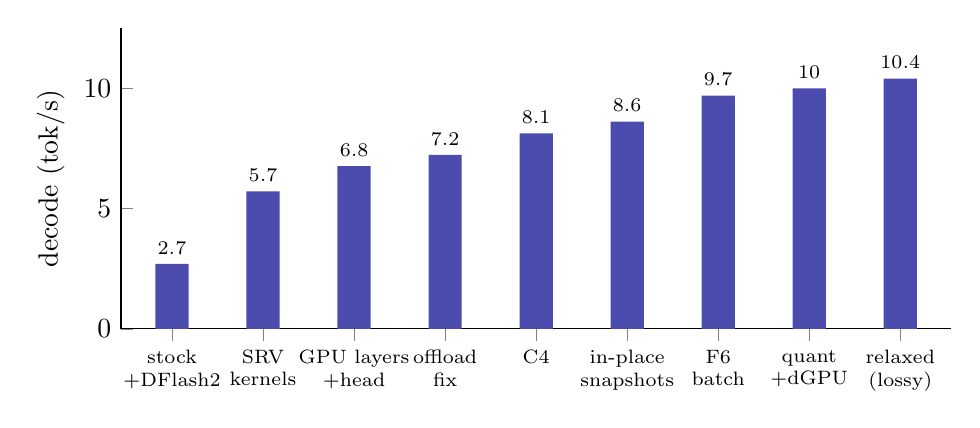
\begin{tikzpicture}
\begin{axis}[ybar, width=\linewidth, height=5.4cm, bar width=12pt, ymin=0, ymax=12.5, ylabel={decode (tok/s)},
  symbolic x coords={a,b,c,d,e,f,g,h,i}, xtick=data, enlarge x limits=0.07,
  xticklabels={{stock\\+DFlash2},{SRV\\kernels},{GPU layers\\+head},{offload\\fix},{C4},{in-place\\snapshots},
               {F6\\batch},{quant\\+dGPU},{relaxed\\(lossy)}},
  xticklabel style={align=center, font=\scriptsize}, nodes near coords, nodes near coords style={font=\scriptsize},
  every node near coord/.append style={/pgf/number format/.cd, fixed, precision=1}, axis x line*=bottom,
  axis y line*=left]
\addplot[fill=blue!55!black!70, draw=none] coordinates {(a,2.70) (b,5.72) (c,6.77) (d,7.23) (e,8.13) (f,8.62) (g,9.70) (h,10.0) (i,10.4)};
\end{axis}
\end{tikzpicture}

\caption{Decode speed of Qwen3.8-27B on the reference laptop as the components are added (10 prompts for F6 steps,
5 for the earlier ones). All configurations up to ``relaxed'' produce the target's greedy output.}
\label{fig:progression}
\end{figure}

Figure~\ref{fig:progression} shows the progression from stock llama.cpp (2.7\,\tps) to 9.6--10.2\,\tps{} with
identical output. The largest steps are the small-batch kernels (2.7$\to$5.7), C4 and in-place snapshots
(7.2$\to$8.6), adaptive drafting and the F6 batch of kernel, rollback and system changes (8.6$\to$9.7), and
kernel-aware quantization and dGPU co-verification (to ${\sim}10$).

\begin{figure}[t]
\centering
% Per-pass wall time vs tokens verified, measured in the server (SRHPM_PASS_LOG)
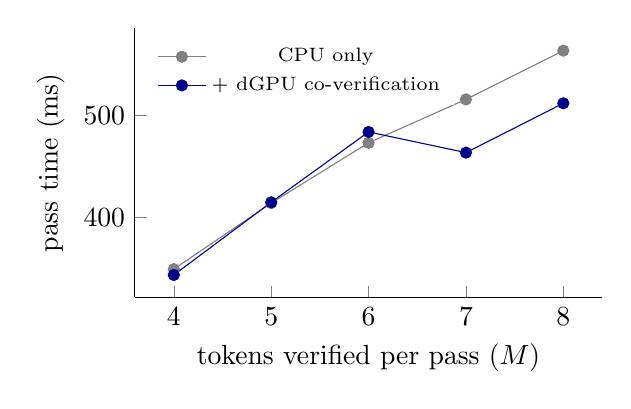
\begin{tikzpicture}
\begin{axis}[width=0.62\linewidth, height=5cm, xlabel={tokens verified per pass ($M$)}, ylabel={pass time (ms)},
  xtick={4,5,6,7,8}, legend style={draw=none, font=\scriptsize, at={(0.03,0.97)}, anchor=north west},
  axis x line*=bottom, axis y line*=left]
\addplot[mark=*, gray] coordinates {(4,349.6) (5,414.1) (6,473.0) (7,515.4) (8,563.0)};
\addplot[mark=*, blue!55!black] coordinates {(4,343.9) (5,414.9) (6,483.6) (7,463.4) (8,511.6)};
\legend{CPU only, + dGPU co-verification}
\end{axis}
\end{tikzpicture}

\caption{Wall time of a verification pass versus tokens verified, measured inside the server during decoding
(\texttt{SRHPM\_PASS\_LOG}), with and without dGPU co-verification.}
\label{fig:cost}
\end{figure}

\paragraph{Where the time goes.} A per-op profile of a pass (${\sim}0.45$\,s) attributes 76\% to the CPU matrix
products (IQ4\_XS 55\%, Q3\_K 27\%), 10\% to other CPU ops (recurrent op 4\%), and 14\% to the GPU layers, the
drafter (11\,ms), feature injection (2\,ms) and fixed overheads. The pass time grows from 0.34\,s at $M=4$ to
0.51\,s at $M=8$ (Figure~\ref{fig:cost}).

\paragraph{Prose.} On summaries of Spanish prose the drafter's acceptance falls to 0.45--0.58 and decoding to
${\sim}6$\,\tps{} on the same hardware: SR-HPM's gains scale with the drafter's quality.

\paragraph{Context window.} The pass time does not grow with context up to 4.8k tokens, but it does beyond.
Table~\ref{tab:ctx} measures windows up to the model's 262k tokens. A q8 KV cache is free in quality (KLD to Q8\_0
0.0428 vs 0.0430 with f16) and halves the cache; kept in system RAM it takes no VRAM from the model's layers. Merely
configuring a large window costs 10\% at 32--128k and 32\% at 262k, where the drafter's own cache exhausts the VRAM.
Filling it costs more, because attention over the whole cache runs on the CPU for every verified token.
With a quantized cache llama.cpp's CPU attention handled each (token, query head) row separately and dequantized the
whole cache for each, 24$\times$ the traffic for 4 tokens and 6 query heads per KV head: 0.5\,\tps{} at 100k tokens.
We extended our grouped small-batch attention to quantized caches: each K row is read once per KV head and multiplied
in int8 against the query rows quantized once per tile (the stock path's arithmetic, so the output is identical), and
each V row is dequantized once. Decode at 100k tokens rises 4.4$\times$ (Table~\ref{tab:ctx}); it is the same idea as
the weight kernels, memory-flat verification, applied to the cache.

\begin{table}[t]
\centering\small
\begin{tabular}{lccc}
\toprule
Tokens in context (128k window, q8 cache in RAM) & time to first token & decode, stock & decode, grouped \\
\midrule
9.7k & 57\,s & 3.4 & 5.2 \\
36k & 3.6\,min & 1.5 & 4.1 \\
63k & 6.6\,min & 0.7 & $\ge$2.5 \\
100k & 11\,min & 0.5 & 2.2 \\
190k (262k window) & 29\,min & 0.24 & -- \\
\bottomrule
\end{tabular}
\caption{Long prompts (summaries of Spanish text, where the drafter is weak). Prompt processing stays at
110--170\,\tps; decode degrades with the tokens actually in context, not with the configured window. ``Stock'':
llama.cpp's CPU attention for quantized caches; ``grouped'': ours (the 63k figure from a version that dequantized K).}
\label{tab:ctx}
\end{table}

\paragraph{Sampling and thinking.} All other numbers are greedy. At temperature~1 (top-$k$ 20, top-$p$ 0.95) decode
drops 9\% (9.6$\to$8.8\,\tps) as sampled tokens match the drafter less often. Probabilistic drafting with rejection
verification, which keeps the sampled distribution exact, does not recover it (8.8--9.0). With the model's reasoning
mode on, 7.5\,\tps.

\paragraph{Generality.} Nothing in the kernels or the launcher is specific to Qwen: the launcher reads any GGUF,
chooses between all-GPU, MoE and SR-HPM paths, and places layers by the measured cost of their tensor types. MoE models
do not benefit---each verified token activates different experts, so verification is not memory-flat.

\paragraph{Integration.} The result is a standard \texttt{llama-server} with an OpenAI-compatible HTTP API, so an
application, agent framework or pipeline uses it by pointing its base URL at the local server; chat, streaming, JSON
grammars and tool calls are unchanged and SR-HPM only affects how fast tokens are produced. It pays off where
generation dominates (assistants, code, writing, agents with moderate prompts). It pays off less, or loses, where long
prompts precede very short answers: prompt processing runs at ${\sim}130$\,\tps{} against ${\sim}220$ for stock
llama.cpp on the reference laptop, because fewer layers stream their weights through the GPU per batch. Requests are
served one at a time.

\section{What did not work}\label{sec:negative}

\begin{table}[t]
\centering\small
\begin{tabular}{p{0.37\linewidth}p{0.55\linewidth}}
\toprule
Idea & Refuting measurement \\
\midrule
Lossless entropy coding of the weights & IQ4\_XS codes carry 3.91 of 4 bits ($\le3\%$) \\
Delta verification $W(x_t-x_0)$ & deltas are 50--95\% of the activation norm \\
SMT helper threads prefetching weights & the kernel is compute-bound with $\ge4$ tokens \\
iGPU as second verifier (OpenCL) & 38\,GB/s alone; 5.5$\times$ slower with the CPU busy (APU power budget) \\
Draft trees / two chains & $\le+3\%$ with the real cost curve; on a recurrent model chains duplicate the prefix \\
Expected-acceptance path over the lattice & $+0.3\%$ $\tau$ \\
Online reranker of the 16 candidates & $\tau$ 4.098 vs 4.105 (a perfect one: 6.33) \\
Logit lens of the GPU layers as reranker & layer 20 picks the right candidate 10.9\% of the time \\
2-bit CPU layers & KLD 0.094 and \emph{slower} (7.8 vs 9.6\,\tps): grid decode is compute-bound \\
Low-rank GPU correction of 2-bit error & residual nearly white: rank 256 removes 10--20\% \\
Sensitivity-guided mix (imatrix-weighted error) & predicted KLD 0.042, measured 0.057; fitted: $-1.8\%$ bytes \\
Pass-shared activation sparsity & skipping 10\% of blocks costs 5--10$\times$ the quantization error \\
Layer dropping & 2 layers: KLD 0.043$\to$0.108 \\
Exact output head on a vocabulary subset & the bound adds 60--95 logits; 97--100\% of the head is read \\
Small ops on one thread, fewer barriers & same speed; cache misses, not barriers \\
N-gram retrieval drafting & never fires on chat or summaries (paraphrase) \\
Probabilistic drafting at temperature 1 & 8.8--9.0 vs 8.8\,\tps{} with greedy drafting \\
More GPU layers in spare VRAM & below ${\sim}0.4$\,GB free, WDDM slows everything down \\
\bottomrule
\end{tabular}
\caption{Refuted ideas. Scripts and data in \texttt{research/}.}
\label{tab:negative}
\end{table}

Table~\ref{tab:negative} lists ideas that failed, including training-free activation sparsity~\cite{teal} and
layer dropping~\cite{shortgpt}. Three findings shape what is left. First, with 4 tokens per pass the
CPU already reads at ${\sim}90\%$ of the measured DRAM ceiling: any further gain at that point must reduce bytes, and
every training-free way of doing so we tried (fewer bits, sparsity, dropping layers, a pruned head) costs more quality
than it saves. Second, the drafting \emph{policy} is exhausted---an oracle that stops each chain exactly at its first
error gains only 9\%---but the drafter's 16 candidates contain the right token at 15--19\% of the positions where its
first choice is wrong, so a perfect selection would raise $\tau$ from 4.1 to 6.3. Telling those candidates apart
without training costs as much as verifying them: the GPU-resident first layers do not know (10.9\%), and trees pay for
the extra rows. Third, quantization quality is not predicted by weight error alone: products that write into the
residual stream are ${\sim}16\times$ more sensitive per unit of weighted error.

\section{Limitations and future work}

The fast kernels need x86-64 with AVX2; VNNI and AMX machines and ARM are untested. Rollback assumes one sequence,
so concurrent requests are queued rather than batched, and prompt processing is slower than in stock llama.cpp.
Decode still degrades with long contexts (2.2\,\tps{} at 100k tokens), where CPU attention over the cache
dominates.
The dGPU co-verifier is implemented for Windows and CUDA. All measurements are on one laptop; desktop CPUs with DDR5
and more VRAM shift the balance (more layers on the GPU, more bandwidth), and Linux frees ${\sim}1$\,GB of VRAM
that WDDM reserves. The two levers left with large margins require training, which is outside the scope of a tool
for existing models: adapting the drafter's candidate selector to the quantized target (the 4.1$\to$6.3 headroom), and
layer dropping with a short healing fine-tune.

\section{Conclusion}

Speculative decoding helps memory-bound CPU inference only if verification is memory-flat. Making it so on a
consumer CPU, and then removing the rollback, prompt-processing, placement and idle-GPU costs that appear next,
turns a 27B dense model on a 6\,GB laptop GPU from 2.7 into ${\sim}10$ tokens per second with identical output. The
remaining distance to 20 is set by DRAM bandwidth and by the drafter, not by the software around them.

\begin{thebibliography}{9}\small
\bibitem{leviathan} Y.~Leviathan, M.~Kalman, Y.~Matias. Fast inference from transformers via speculative decoding.
ICML 2023.
\bibitem{chen} C.~Chen et al. Accelerating large language model decoding with speculative sampling. arXiv:2302.01318,
2023.
\bibitem{llamacpp} G.~Gerganov et al. llama.cpp. \url{https://github.com/ggml-org/llama.cpp}.
\bibitem{teal} J.~Liu et al. Training-free activation sparsity in large language models (TEAL). ICLR 2025.
\bibitem{shortgpt} X.~Men et al. ShortGPT: layers in large language models are more redundant than you expect. 2024.
\bibitem{eagle} Y.~Li et al. EAGLE: speculative sampling requires rethinking feature uncertainty. ICML 2024.
\end{thebibliography}

\end{document}
